\section{Results, Demonstration and Discussion}
\label{ch:results}

\subsection{Implemented Features}
Table~\ref{tab:features} lists what was implemented, what is partial and what was not built, with the evidence for each.
\begin{table}[!htbp]
\caption{Feature status}
\label{tab:features}
\footnotesize
\begin{tabularx}{\textwidth}{@{}>{\raggedright\arraybackslash}p{6.0cm}>{\raggedright\arraybackslash}p{2.2cm}>{\raggedright\arraybackslash}X@{}}
\toprule
\textbf{Feature} & \textbf{Status} & \textbf{Evidence}\\ \midrule
Discovery, link-state gossip, weighted Dijkstra, priority, TTL and dedup, ACK and retry, store-and-forward, AES-GCM, Ed25519, SQLite log & Implemented & \NTests\ tests; Chapters~\ref{ch:perf}, \ref{ch:test}\\
Simulator, metrics, API, engine web application, survivor and rescue screens & Implemented & 7 scenarios to 65 nodes; 12 API tests; Section~\ref{sec:shots}\\
Multi-device deployment over real sockets & Implemented & 5 processes measured; two-laptop demonstration\\
Immediate flush on a new neighbour; history filter & Partial & SNF-3, LOG-5\\
BLE or Wi-Fi Direct radio; per-pair key agreement; timed usability study & Not implemented & out of scope or future work\\
\bottomrule
\end{tabularx}
\end{table}

\subsection{Screenshots and Demonstration Evidence}
\label{sec:shots}
All screenshots are from the running system. Figures~\ref{fig:survivor} and~\ref{fig:console} come from the five-process live deployment in the demonstrated story: an SOS is delivered over a relay; the gateway fails and the next SOS is held; the gateway returns and the held message is delivered.
\begin{figure}[!htbp]
\centering
\begin{minipage}[t]{0.22\textwidth}\centering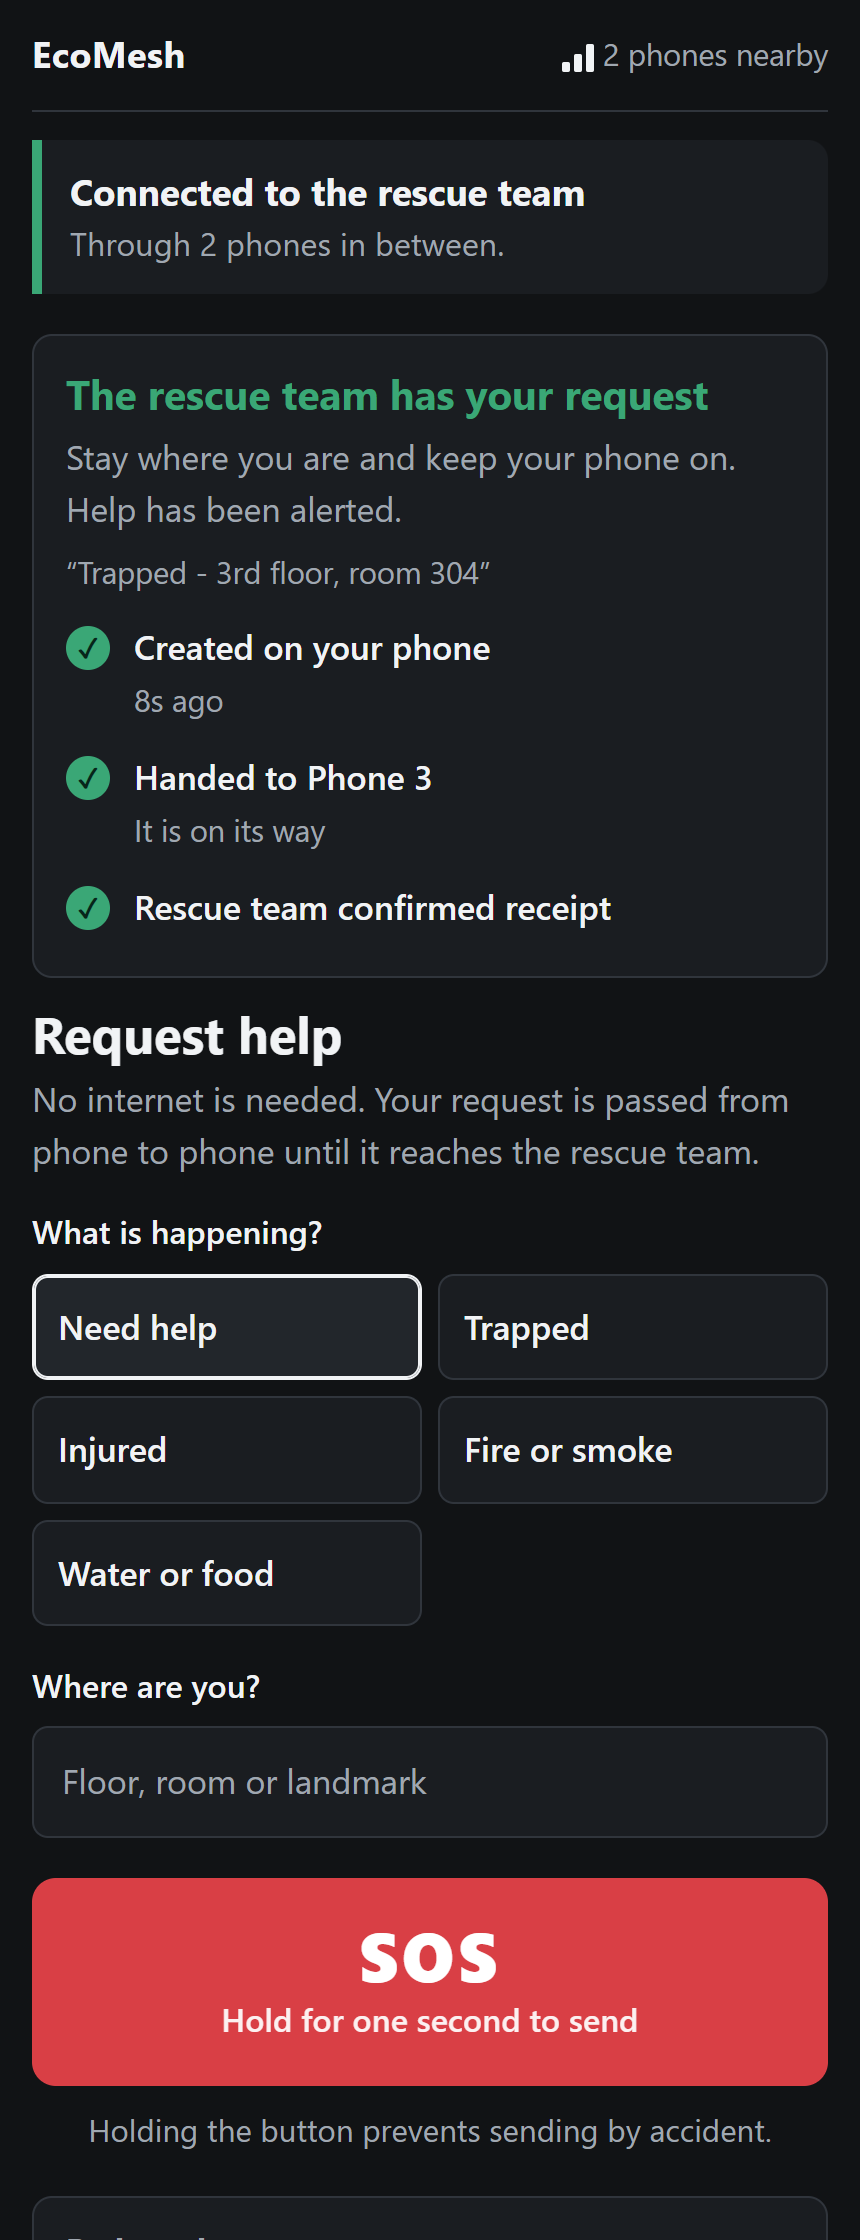
\includegraphics[width=\textwidth]{figures/story_survivor_delivered.png}\end{minipage}\hfill
\begin{minipage}[t]{0.22\textwidth}\centering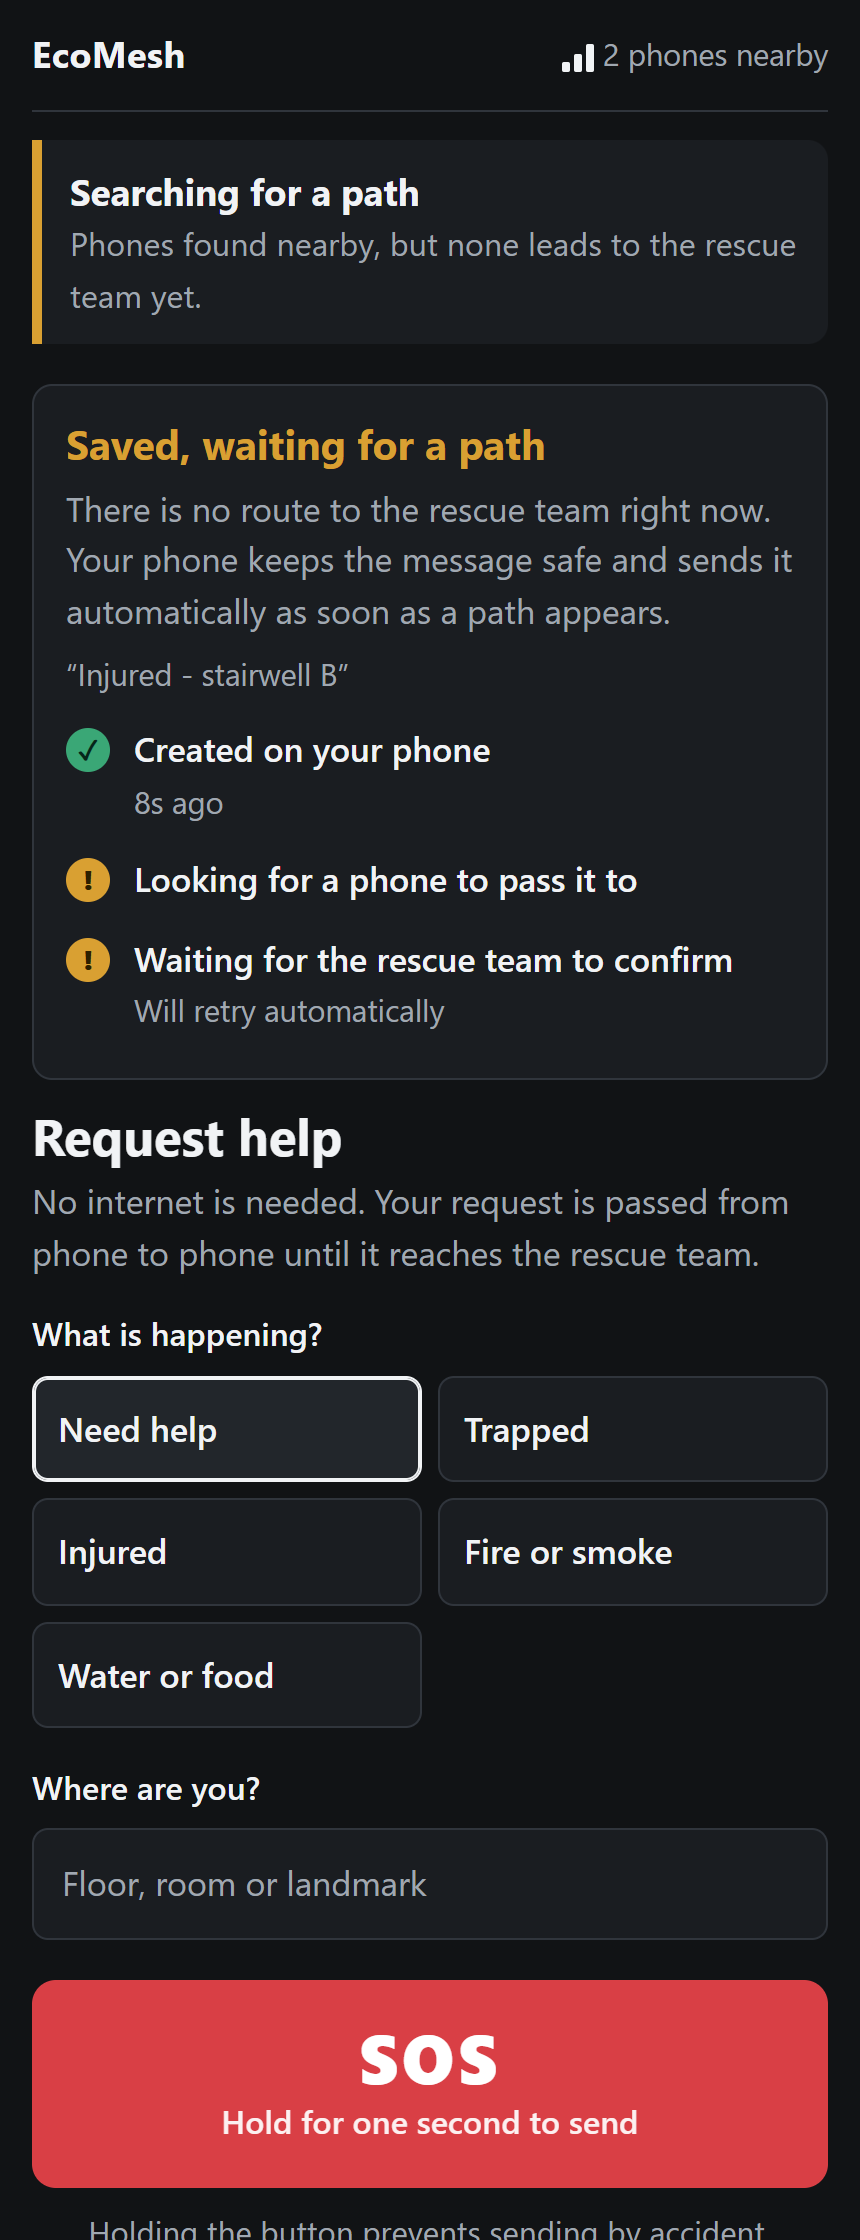
\includegraphics[width=\textwidth]{figures/story_survivor_held.png}\end{minipage}\hfill
\begin{minipage}[t]{0.22\textwidth}\centering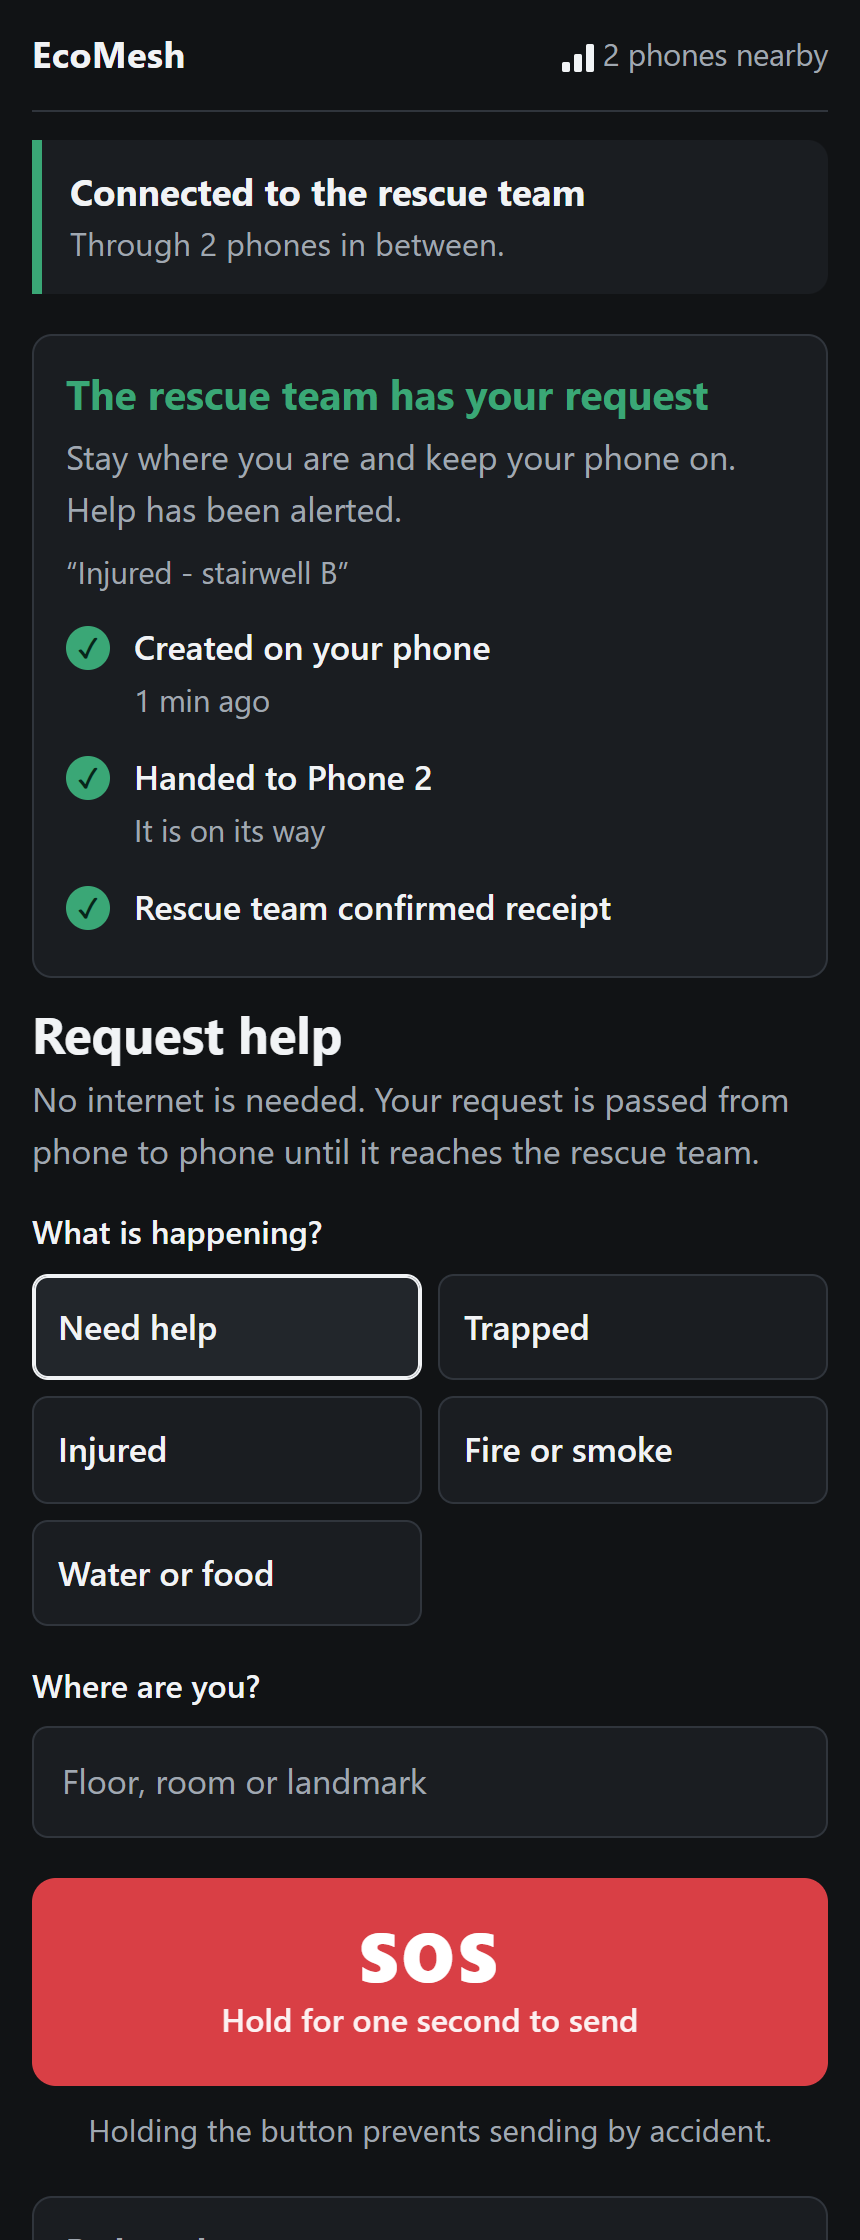
\includegraphics[width=\textwidth]{figures/story_survivor_flushed.png}\end{minipage}
\caption[The survivor's screen: delivered, held and flushed]{The survivor's screen. Left: SOS delivered over a relay phone and the Gateway. Centre: the gateway has failed; the screen says ``Searching for a path'' and the message is ``Saved, waiting for a path''. Right: the gateway is back and the held message is delivered.}
\label{fig:survivor}
\end{figure}
\begin{figure}[!htbp]
\centering
\begin{minipage}[t]{0.43\textwidth}\centering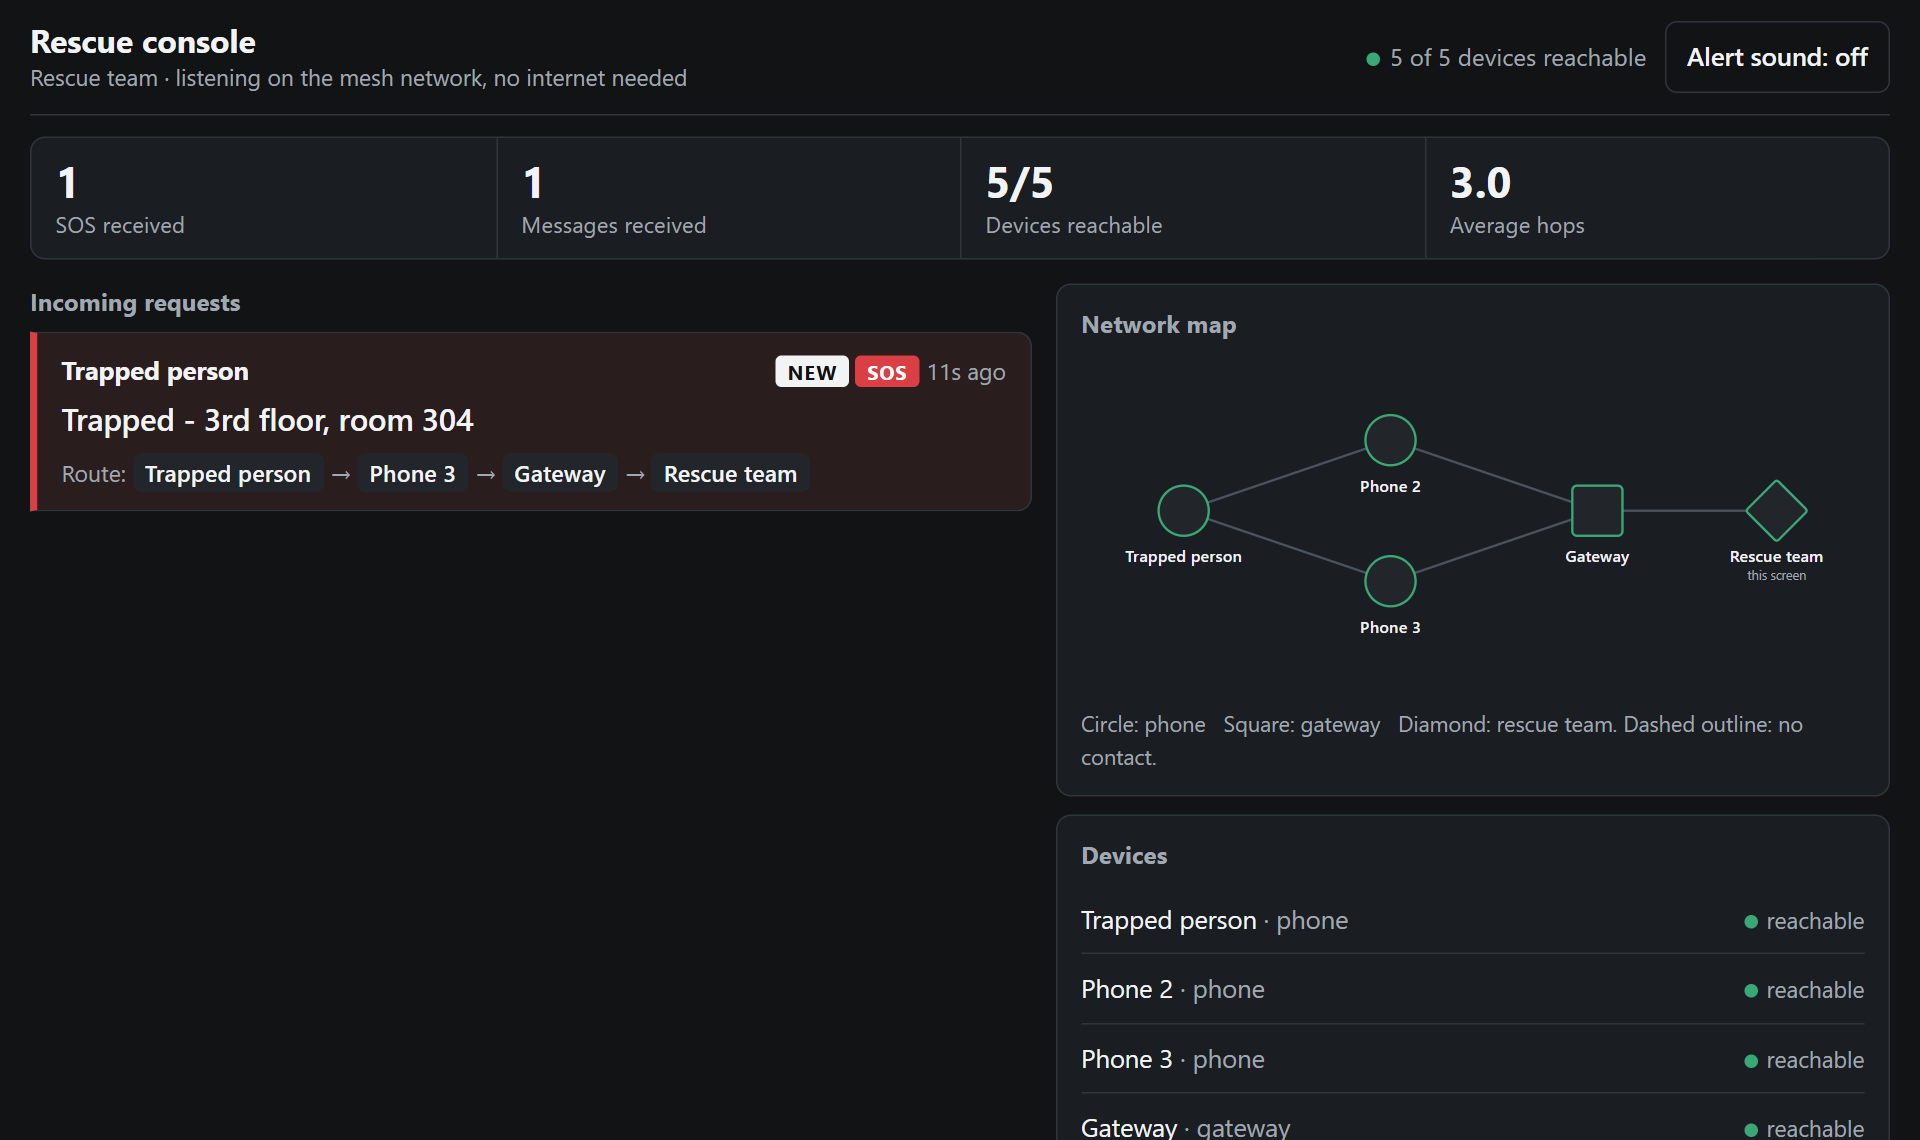
\includegraphics[width=\textwidth]{figures/story_rescue_console.png}\end{minipage}\hfill
\begin{minipage}[t]{0.43\textwidth}\centering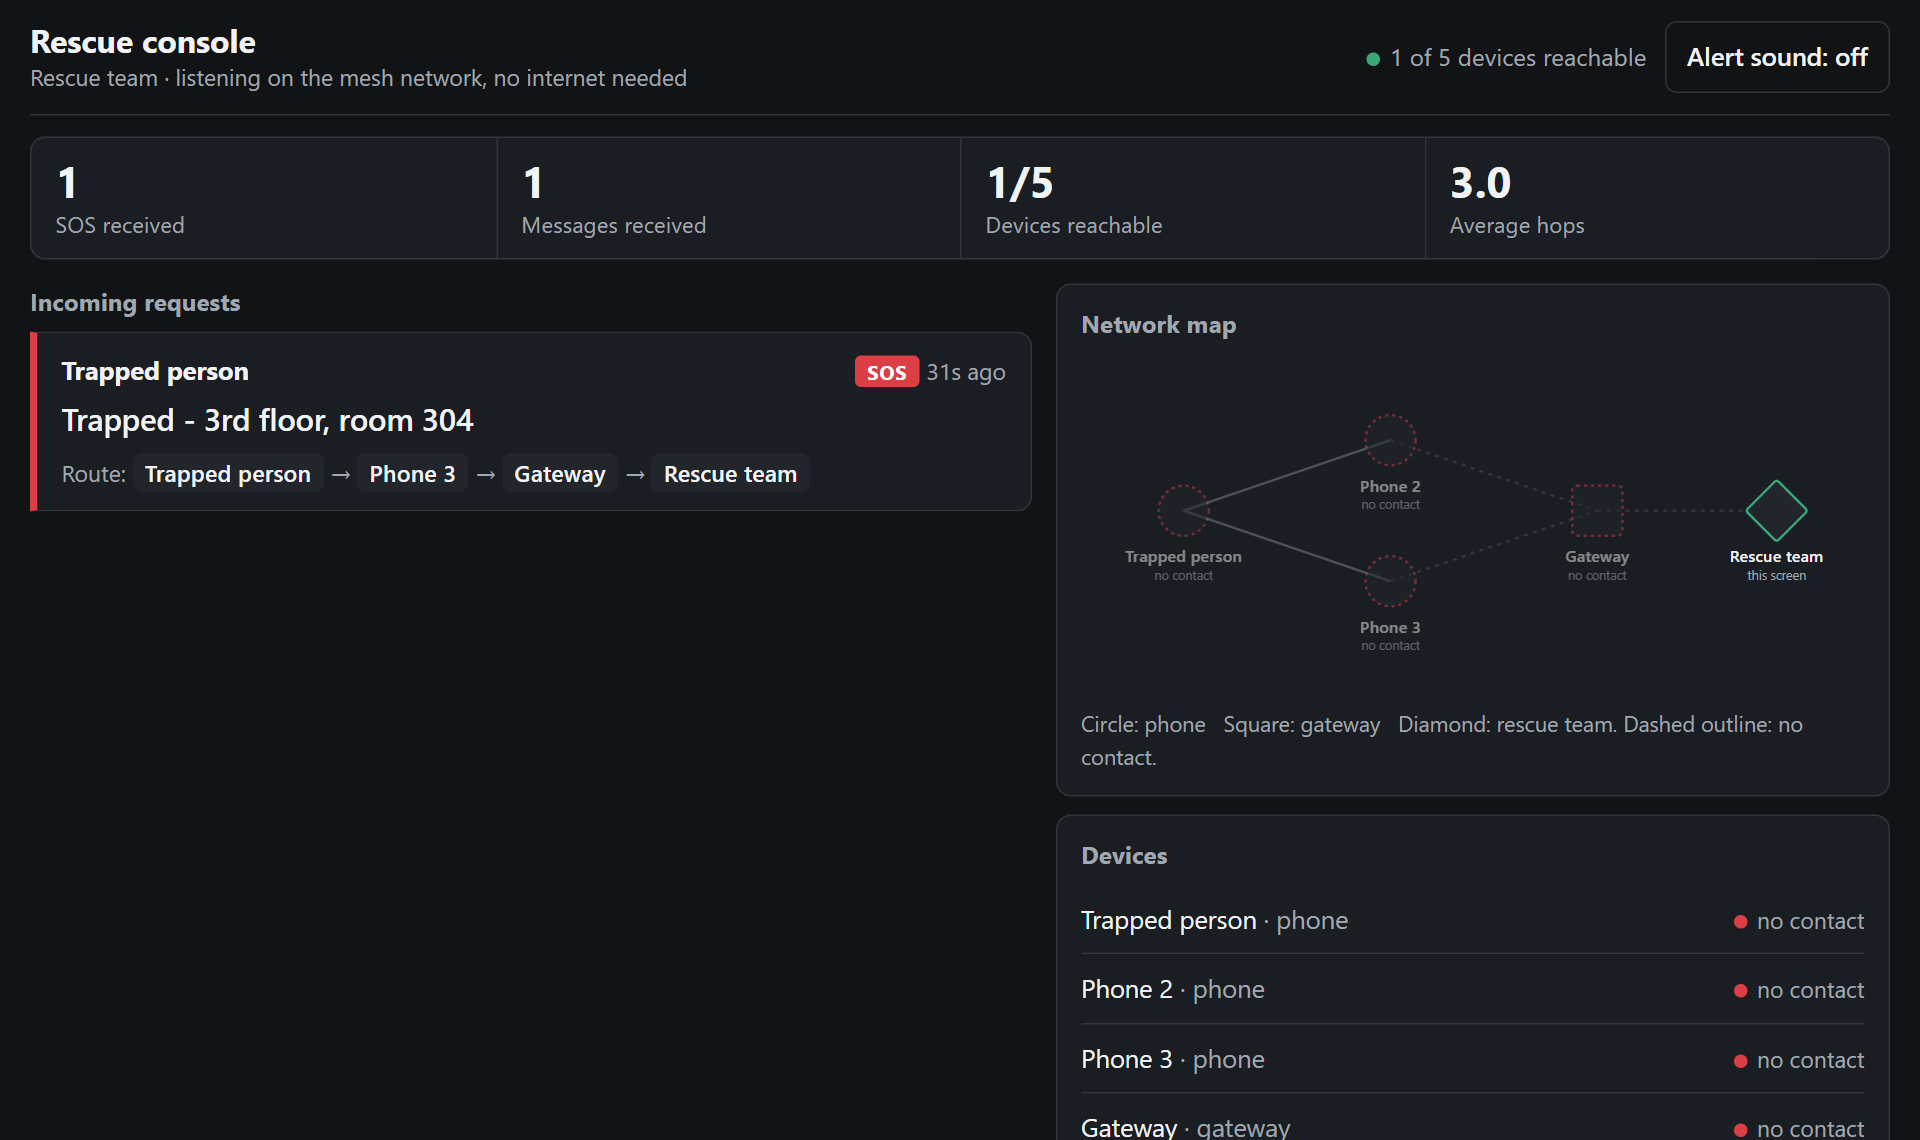
\includegraphics[width=\textwidth]{figures/story_rescue_console_gwdown.png}\end{minipage}
\caption[The rescue console, before and during a gateway outage]{The rescue console. Left: SOS cards with sender, text, age and route, counters, network map and device list. Right: with the gateway down the rescue device hears nobody (``1 of 5 devices reachable''); earlier messages remain visible.}
\label{fig:console}
\end{figure}
\begin{figure}[!htbp]
\centering
\begin{minipage}[t]{0.42\textwidth}\centering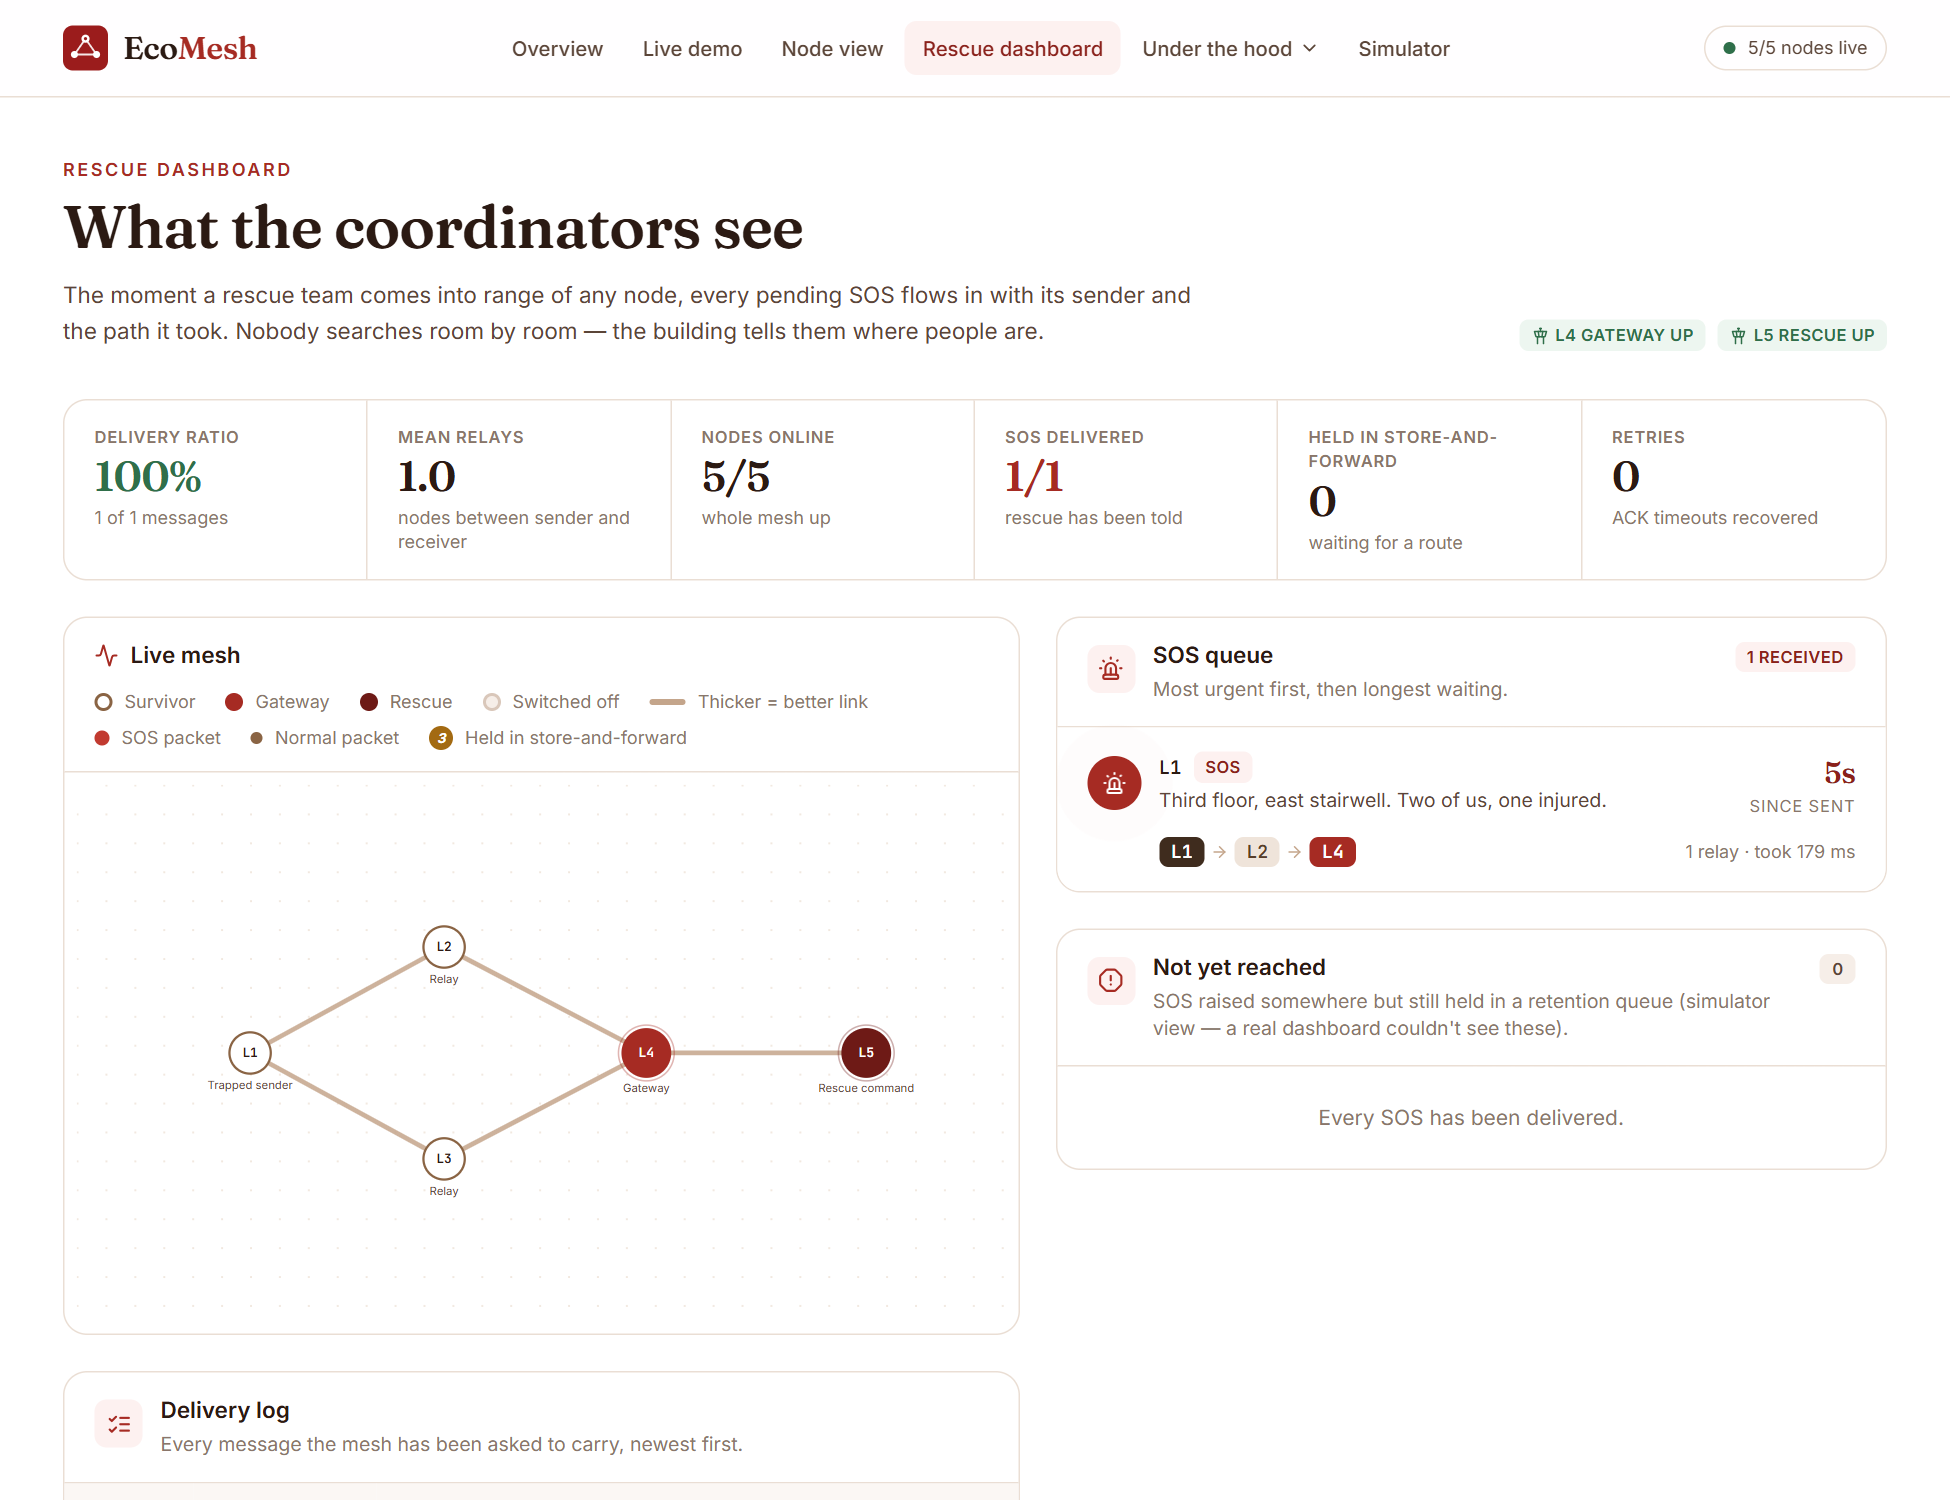
\includegraphics[width=\textwidth]{figures/ui_rescue.png}\end{minipage}\hfill
\begin{minipage}[t]{0.42\textwidth}\centering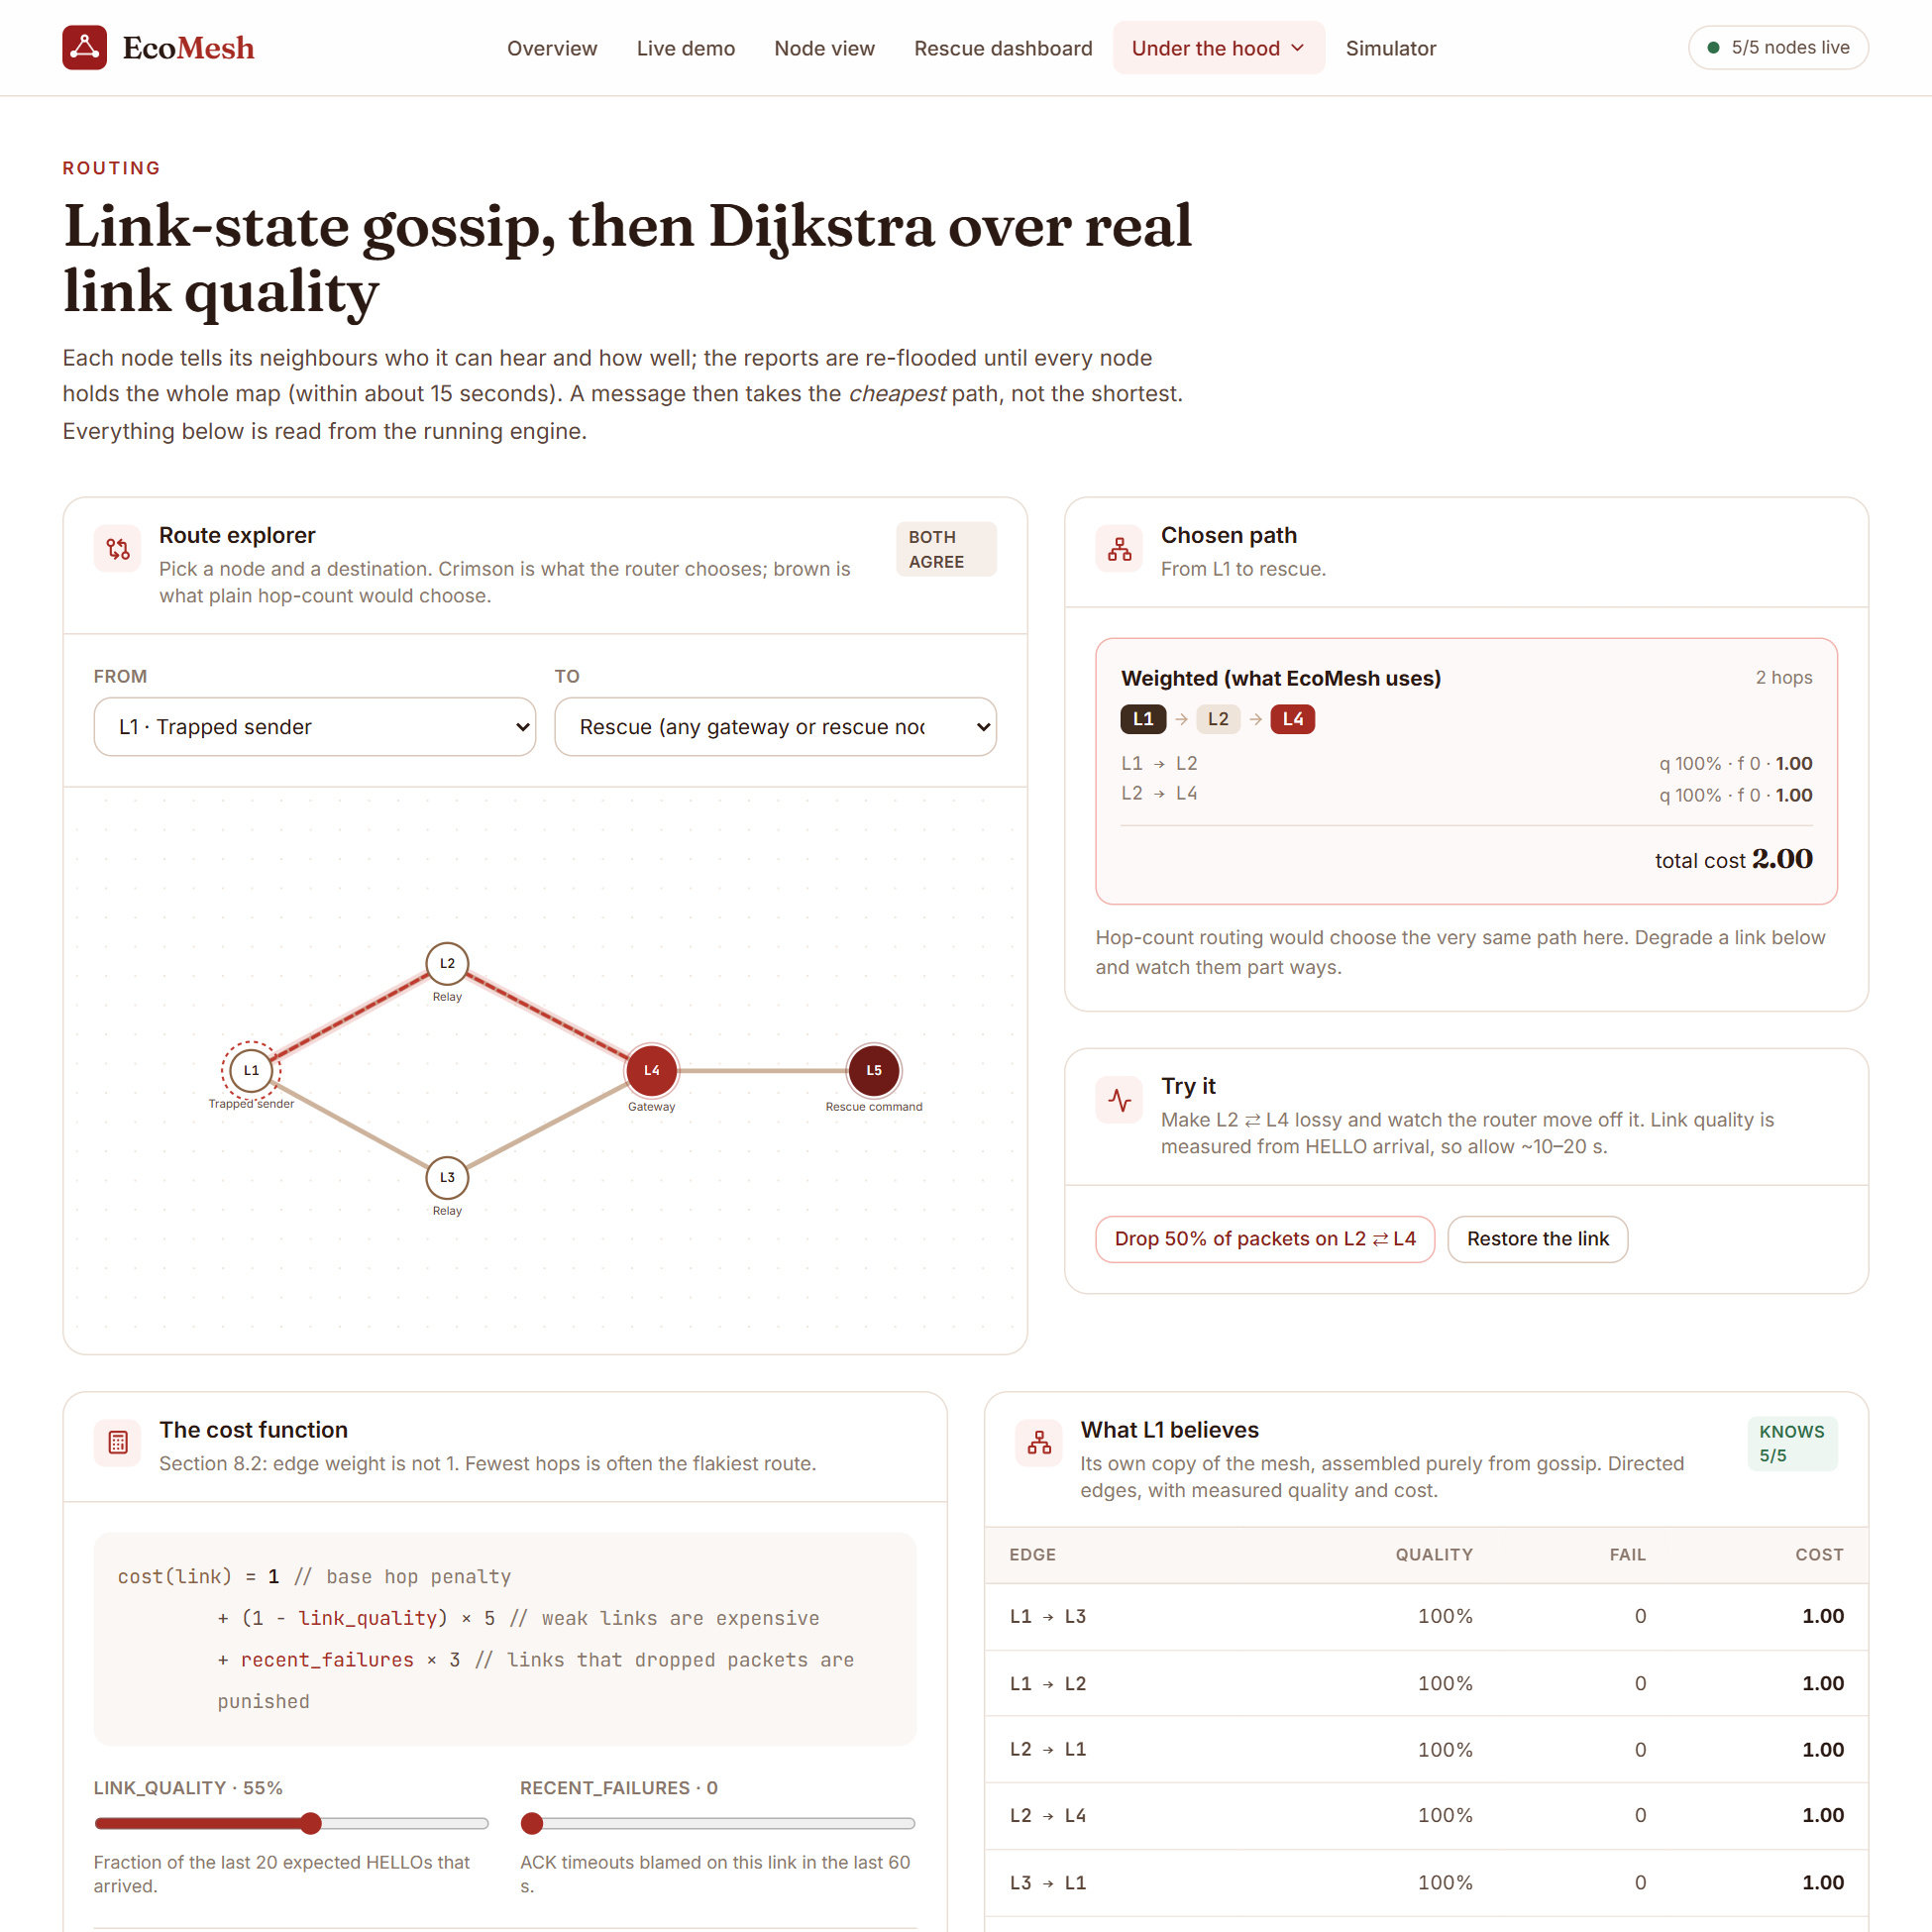
\includegraphics[width=\textwidth]{figures/ui_routing.png}\end{minipage}
\caption[The engine web application: rescue dashboard and routing page]{The engine web application. Left: rescue dashboard (delivery ratio, nodes online, live mesh, SOS queue). Right: routing page (weighted versus hop-count route, cost function, a node's view of the graph). A six-beat live demonstration page drives the same API.}
\label{fig:uishots}
\end{figure}
The mesh was also run on two physical laptops joined by a phone hotspot (Figure~\ref{fig:deploy}): an SOS was delivered across both machines, the route changed when a relay was switched off, and a message held while the gateway was off was delivered when it returned. This run was a functional demonstration and was not timed.

\subsection{Functional Results}
Of the 68 requirements, \NAuto\ are verified by automated tests alone, \NAutoUI\ with a manual screen check, \NInspect\ by inspection, \NManual\ manually, and \NPartial\ are partial (Table~\ref{tab:frsum}). The three key stories ran on real devices: an SOS reaches rescue over several hops, the mesh re-routes around a failed relay, and a message with no route is held and later delivered.
\subsection{Performance Results}
Table~\ref{tab:kpival} collects the measured KPIs: \CollDel\,\% delivery on 40 nodes at 20\,\% loss with failures, an SOS \SosAdv$\times$ faster under load, live SOS delivery in a median 47\,ms, relay failover in about 4\,s and held messages flushed in about 4.5\,s.
\subsection{Comparison with Existing Systems}
Other systems were not run, so the comparison uses documented properties (Table~\ref{tab:compare1}) and the one fair measurable baseline, hop-count routing on identical seeds (\HopW\,\% against \HopH\,\%). No claim is made about the delivery of Bridgefy, Briar, Meshtastic or Serval, which publish no comparable measurements.
\subsection{Achievement of Objectives}
Table~\ref{tab:objectives} maps each objective of Section~1.4 to its evidence and status.
\begin{table}[!htbp]
\caption{Objectives, supporting evidence and status}
\label{tab:objectives}
\footnotesize
\begin{tabularx}{\textwidth}{@{}>{\raggedright\arraybackslash}p{0.9cm}>{\raggedright\arraybackslash}X>{\raggedright\arraybackslash}p{3.4cm}@{}}
\toprule
\textbf{Obj.} & \textbf{Evidence} & \textbf{Status}\\ \midrule
O1 & live convergence 3.8\,s; simulator 5--15\,s in multiples of the gossip interval & Achieved (47 of 50 runs $\le$ 15\,s)\\
O2 & \HopW\,\% vs \HopH\,\% on \HopRuns\ identical seeds (Figure~\ref{fig:results}b) & Achieved\\
O3 & \SosAdv$\times$ lower median latency under load (Section~\ref{sec:perfresults}) & Achieved\\
O4 & \CollDel\,\% at 40 nodes and 20\,\% loss; recovery mean \CollRecMean\,s, \CollRecOK\ of \CollRecN\ trials within 10\,s & Partly achieved\\
O5 & 201 of 201 flushed in simulation; 4 of 4 live outages & Achieved\\
O6 & security tests (Section~\ref{sec:nonfunc}) & Achieved with a pre-shared key\\
O7 & every metric is a query over per-node logs & Achieved\\
O8 & web application, device screens, API tests, five processes, two laptops & Achieved\\
\bottomrule
\end{tabularx}
\end{table}

\subsection{Discussion of Findings}
Hop count is a poor proxy for delivery: a weak shortcut loses almost half the traffic under hop count and almost none under the weighted cost. Timer constants, not algorithms, set recovery and convergence (they cluster at the heartbeat timeout and the gossip interval), which shows exactly what to tune. Loss is paid for in tail latency, and priority matters only once a link queues, which is the disaster condition. Testing found real defects in code we believed finished (Section~\ref{sec:defects}).

\subsection{Practical Applicability}
A deployment needs devices running the node program, a topology file (or multicast discovery), a gateway or rescue device and a shared network segment. It is usable today as a campus, hospital or building safety system on laptops; a Bluetooth LE or Wi-Fi Direct transport would make it phone-to-phone.
